\documentclass[tikz,border=6pt]{standalone}
\usepackage{amsmath}
\usepackage{newtxtext,newtxmath}
\usetikzlibrary{arrows.meta,calc}

\begin{document}
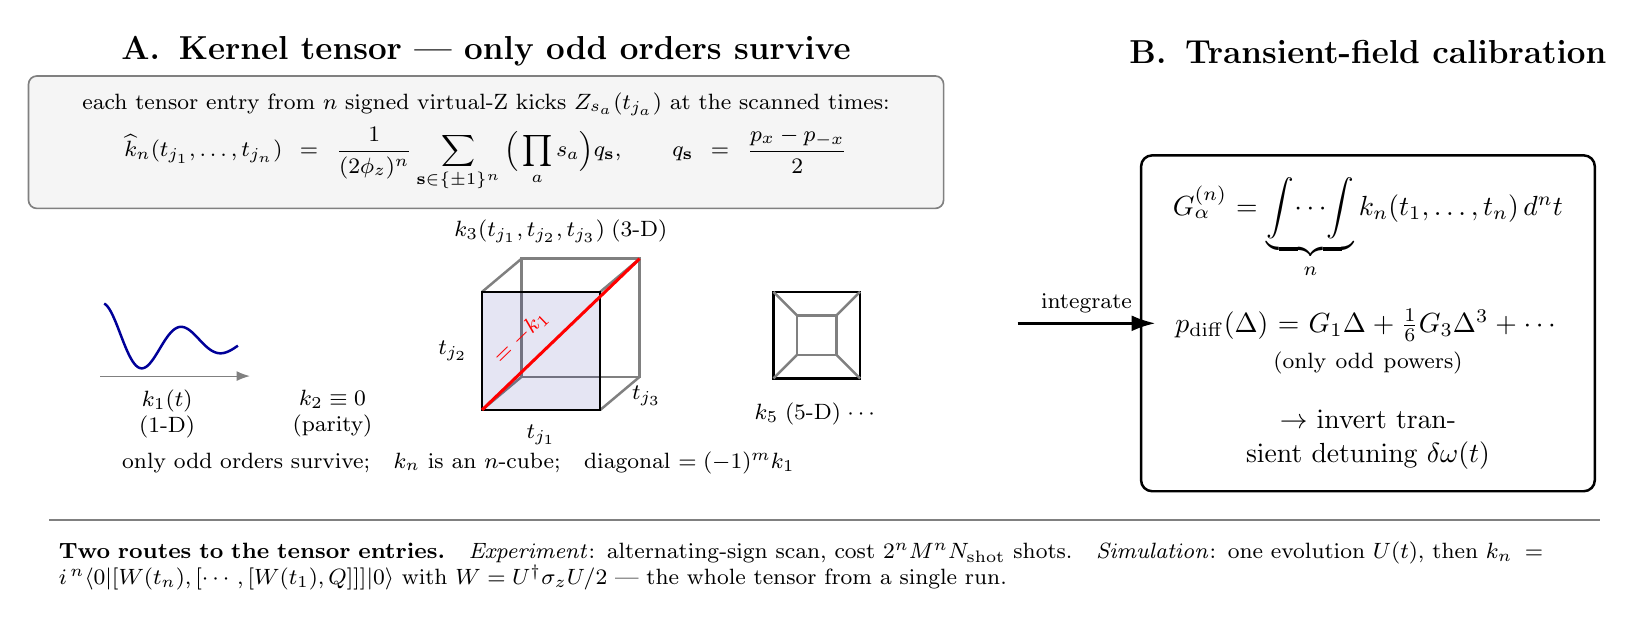
\begin{tikzpicture}[
  x=1cm,y=1cm,>=Latex,font=\normalsize,
  line/.style={draw=black,line width=0.9pt},
  arrow/.style={line,-{Latex[length=3mm,width=2mm]}},
  panel/.style={draw=black,line width=0.9pt,rounded corners=4pt,align=center,inner sep=8pt},
  caption/.style={draw=gray,line width=0.6pt,rounded corners=3pt,fill=black!4,align=center,
                  font=\footnotesize,inner sep=6pt}
]

% ===================== titles =====================
\node[font=\bfseries\large] at (5.55,3.60) {A.\, Kernel tensor --- only odd orders survive};
\node[font=\bfseries\large] at (16.75,3.60) {B.\, Transient-field calibration};

% ===================== folded estimator (was block A) =====================
\node[caption,text width=11.2cm] at (5.55,2.45)
  {each tensor entry from $n$ signed virtual-Z kicks $Z_{s_a}(t_{j_a})$ at the scanned times:\\[3pt]
   $\widehat{k}_n(t_{j_1},\dots,t_{j_n})=\dfrac{1}{(2\phi_z)^{n}}
   \displaystyle\sum_{\mathbf{s}\in\{\pm1\}^{n}}\Big(\prod_a s_a\Big)q_{\mathbf{s}},
   \qquad q_{\mathbf{s}}=\dfrac{p_x-p_{-x}}{2}$};

% ===================== B: the order ladder =====================
% --- k1 : a 1-D curve ---
\begin{scope}[shift={(0.70,-0.10)}]
  \draw[->,gray] (-0.05,-0.42) -- (1.85,-0.42);
  \draw[blue!60!black,line width=0.9pt,domain=0:1.7,samples=90,smooth]
    plot (\x,{0.50*exp(-0.9*\x)*cos(360*\x)});
\end{scope}
\node[font=\footnotesize,align=center] at (1.50,-1.00) {$k_1(t)$\\(1-D)};

% --- k2 : vanishes by parity ---
\node[font=\Large,gray] at (3.60,-0.02) {$\varnothing$};
\node[font=\footnotesize,align=center] at (3.60,-1.00) {$k_2\equiv0$\\(parity)};

% --- k3 : a 3-D cube with red space diagonal ---
\begin{scope}[shift={(5.50,-0.95)}]
  \def\L{1.5}\def\dx{0.50}\def\dy{0.42}
  \draw[line,draw=gray] (\dx,\dy) -- (\L+\dx,\dy) -- (\L+\dx,\L+\dy) -- (\dx,\L+\dy) -- cycle;
  \draw[line,draw=gray] (0,0)--(\dx,\dy);
  \draw[line,draw=gray] (\L,0)--(\L+\dx,\dy);
  \draw[line,draw=gray] (\L,\L)--(\L+\dx,\L+\dy);
  \draw[line,draw=gray] (0,\L)--(\dx,\L+\dy);
  \fill[blue!55!black,opacity=0.10] (0,0) rectangle (\L,\L);
  \draw[line] (0,0) -- (\L,0) -- (\L,\L) -- (0,\L) -- cycle;
  \draw[red,line width=1.1pt] (0,0) -- (\L+\dx,\L+\dy);
  \node[font=\footnotesize,anchor=north] at (0.5*\L,-0.06) {$t_{j_1}$};
  \node[font=\footnotesize,anchor=east]  at (-0.06,0.5*\L) {$t_{j_2}$};
  \node[font=\footnotesize,anchor=west]  at (\L+0.5*\dx+0.03,0.5*\dy-0.03) {$t_{j_3}$};
  \node[red,font=\footnotesize,anchor=south,rotate=44] at (0.44*\L,0.50*\L) {$=-k_1$};
\end{scope}
\node[font=\footnotesize,anchor=south] at (6.50,1.05) {$k_3(t_{j_1},t_{j_2},t_{j_3})$\;(3-D)};

% --- k5 : abstract hypercube icon ---
\begin{scope}[shift={(9.20,-0.55)}]
  \draw[line] (0,0) rectangle (1.1,1.1);
  \draw[line,draw=gray] (0.30,0.30) rectangle (0.80,0.80);
  \draw[line,draw=gray] (0,0)--(0.30,0.30);
  \draw[line,draw=gray] (1.1,0)--(0.80,0.30);
  \draw[line,draw=gray] (1.1,1.1)--(0.80,0.80);
  \draw[line,draw=gray] (0,1.1)--(0.30,0.80);
\end{scope}
\node[font=\footnotesize,align=center] at (9.75,-1.00) {$k_5$\;(5-D)\;$\cdots$};

% --- ladder summary ---
\node[font=\footnotesize,align=center] at (5.20,-1.62)
  {only odd orders survive;\quad $k_n$ is an $n$-cube;\quad diagonal $=(-1)^{m}k_1$};

% ===================== arrow B -> C =====================
\draw[arrow] (12.30,0.15) -- node[above,font=\footnotesize] {integrate} (14.05,0.15);

% ===================== C: calibration =====================
\node[panel,text width=5.2cm] (calib) at (16.75,0.15)
  {$G_\alpha^{(n)}=\underbrace{\int\!\cdots\!\int}_{n} k_n(t_1,\dots,t_n)\,d^{n}t$\\[10pt]
   $p_{\mathrm{diff}}(\Delta)=G_1\Delta+\tfrac16 G_3\Delta^3+\cdots$\\[1pt]
   {\footnotesize(only odd powers)}\\[10pt]
   $\rightarrow$ invert transient detuning $\delta\omega(t)$};

% ===================== footer: the two routes =====================
\draw[gray,line width=0.5pt] (0.0,-2.35) -- (19.7,-2.35);
\node[anchor=north west,font=\footnotesize,text width=19.4cm,align=left] at (0.0,-2.50)
  {\textbf{Two routes to the tensor entries.}\quad
   \emph{Experiment}: alternating-sign scan, cost $2^{n}M^{n}N_{\mathrm{shot}}$ shots.\quad
   \emph{Simulation}: one evolution $U(t)$, then
   $k_n=i^{\,n}\langle0|[W(t_n),[\cdots,[W(t_1),Q]]]|0\rangle$ with
   $W=U^{\dagger}\sigma_z U/2$ --- the whole tensor from a single run.};

\end{tikzpicture}
\end{document}
